%We propose a hardware and software solution to overcome the performance bottleneck described in the previous section. 
%In our system we assume the existence of a specialized hardware that is responsible for the fast execution of the task creation. 
%To use such a hardware we need flexible software that manages to move the task creation to be executed there.

%The software that we employ uses a specialized queue for the task creation requests. 
%Each thread that is about to create a task instead of creating it, it inserts a task creation request in this queue. 
%The responsible hardware then reads the queue and executes the requests.

In this paper we propose a semi-centralized runtime system that dynamically separates the most computationally intensive parts of the runtime system and accelerates them on specialized hardware. 
To develop the {\proposal} we use the OpenMP programming model~\cite{OpenMP},~\cite{OpenMP4.0:Manual2013}.
The base of our implementation is the Nanos++ runtime system responsible for the parallel execution.

Nanos++ is a distributed runtime system that uses dynamic scheduling.
As most task-based programming models, Nanos++ consists of the master and the worker threads.
The master thread is launching the parallel region and creates the tasks that have been defined by the programmer{\footnote{Nanos++ also supports nested parallelism so any of the worker threads can potentially create tasks. However the majority of the existing parallel applications are not implemented using nested parallelism.}}.
The scheduler of Nanos++ consists of a~\textit{ready queue} (\textit{TaskQ}) that is shared for reading and writing among threads and is used to keep the tasks that are ready for execution.
All threads have access to the \textit{TaskQ} and once they become available they try to pop a task from the \textit{TaskQ}.
When a thread finishes a task, it performs all the essential steps described in Section~\ref{sec.background} to keep the data dependency structures consistent.
Moreover, it pushes the tasks that become ready to the \textit{TaskQ}.

%We implement the Runtime Activity Manager ({\proposal}) on top of Nanos distributed runtime system that uses dynamic scheduling~\cite.


\subsection{Implementation}

{\proposal} relieves the master and worker threads from the intensive work of task creation by offloading it on the specialized hardware.
%{\proposal} assumes the existence of a specialized hardware that accelerates this part of the runtime.
Our runtime, apart from the master and the worker threads, introduces the Special Runtime Thread (SRT). 
When the runtime system starts, it creates the SRT and binds it to the task creation accelerator, keeping its thread identifier in order to manage the usage of it.
During runtime, the master and worker threads look for ready tasks in the task ready queue and execute them along with the runtime.
Instead of querying the ready queue for tasks, the SRT looks for runtime activity requests in the Runtime Requests Queue (\textit{RRQ}) and if there are requests, it executes them.

Figure~\ref{fig:communication} shows the communication infrastructure between threads within {\proposal}.
Our system maintains two queues; the Ready Task Queue (\textit{TaskQ}) and the Runtime Requests Queue (\textit{RRQ}).
The \textit{TaskQ} is used to keep the tasks that are ready for execution. 
The \textit{RRQ} is used to keep the pending runtime activity requests. 
The master and the worker threads can push and pop tasks to and from the \textit{TaskQ} and they can also add runtime activity to the \textit{RRQ}. 
The special runtime thread (SRT) pops runtime requests from the \textit{RRQ} and executes them on the accelerator.

When the master thread encounters a task clause in the application's code, after allocating the memory needed, it calls the \texttt{createTask} as shown in Listing~\ref{taskCreation} and described in Section~\ref{sec.background}. 
{\proposal} decouples the execution of \texttt{createTask} from the master thread. 
To do so, {\proposal} implements a wrapper function that is invoked instead of \texttt{createTask}.
In this function, the runtime system checks if the SRT is enabled; if not then the default behaviour takes place, that is, to perform the creation of the task.
If the SRT is enabled, a \textit{Create} request is generated and inserted in the \textit{RRQ}.
The \textit{Create} runtime request includes the appropriate info to execute the code described in Listing~\ref{taskCreation}.
That is, the dependence analysis data, the address of the allocated task, its parent and its arguments.


\begin{lstlisting}[float, emph={void,if,return,non_critical_queue, critical_queue,not,true,and,break}, captionpos=b, caption={Pseudo-code for the SRT loop.},label=SRTloop, emph={[2]mat}, emphstyle={[2]}, aboveskip={0\baselineskip}, frame=tb, belowskip={0\baselineskip}]
1 void SRTloop() {
2  while( true ) {   
3    while(RRQ is not empty) {
4      executeRequest( RRQ.pop() );
5  }
6  if( runtime.SRTstop() ) break;
7 return; 
8}  
\end{lstlisting}

While the master and worker threads are executing tasks, the SRT is looking for \textit{Create} requests in the \textit{RRQ} to execute.
Listing~\ref{SRTloop} shows the code that the SRT is executing until the end of the parallel execution.
The special runtime thread continuously checks whether there are requests in the \textit{RRQ} (line 3). 
If there is a pending creation request, the SRT calls the \texttt{executeRequest} (line 4), which extracts the appropriate task creation data from the creation request and performs the task creation by calling the \texttt{createTask} described in Listing~\ref{taskCreation}.
%executes the task submission and inserts the task in the TDG with a call to the \texttt{executeRequest} (line 4). 
When the parallel region is over, the runtime system informs the SRT to stop execution.
This is when the SRT exits and the execution finishes (line 6).

%\kc{communication:} To relieve the master and worker threads from the intensive runtime activity we use a simple queueing communication scheme that offloads the task submission on a specialized hardware.
%Whenever a thread encounters a task submission phase, instead of executing the submit call of the scheduler, it creates a runtime request and inserts it in the RRQ. 
%Concurrently, the SRT queries the RRQ for runtime requests and as long as there are requests available it executes them.
%Moreover, the SRT executes tasks whenever there are no requests for a long time to speedup the execution.

\begin{figure}[t]%
	\centering
	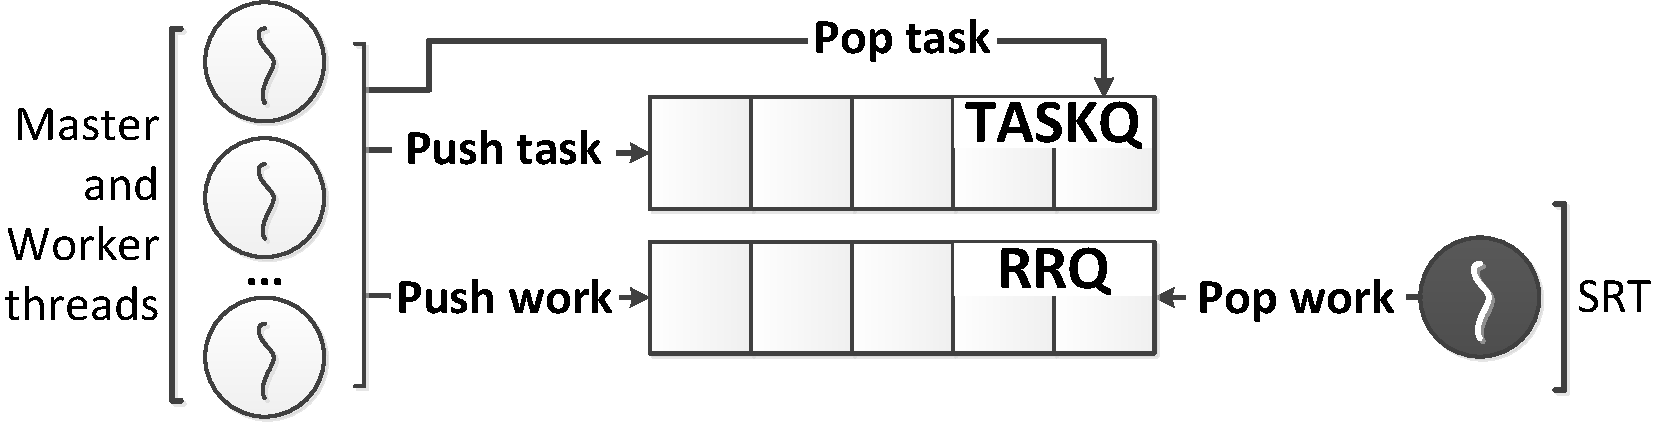
\includegraphics[width=1.0\columnwidth]{figures/communication2.pdf}
	\vspace{-0.5cm}
	\caption{Communication mechanism between master/workers and SRT threads.}
	\label{fig:communication}%
	\vspace{-0.3cm}
\end{figure}




